\chapter{$ \scheme $ Construction}
\label{chap:constr}

\begin{quote} \small
	We will see the construction of $ \scheme $.
\end{quote}

\section{Construction}

We have with us the following:
\begin{itemize}
	\item A metric space ($\msgspc$, $\mathsf{dis}$)  with hamming distance as the distance metric.
	\item An $(l,m,\kappa,\epsilon)$-strong extractor.
	\item An error-correcting code $C = (\msgspc, K, \tau)$.
	\item A collision resistant hash function family $\mathsf{H}=(\mathcal{HK, H})$.
	\item $\mathsf{SE = (E,D)}$ denotes a symmetric encryption scheme.
\end{itemize}

The $\scheme [C, \mathsf{H}, \mathsf{SE}]$ is defined by one procedure - $\mathsf{Init}$ - and three protocols - $\mathsf{Reg}$, $\mathsf{Put}$ and $\mathsf{Get}$. The server maintains three tables:
\begin{itemize}
	\item $\textbf{fil}$: which contains the encryptions of the files uploaded by the clients. Each ciphertext in this table is indexed using a unique identifier derived from itself which we call the $tag$. This table is immutable.
	\item $\textbf{delt}$: which stores the $\Delta$ as discussed in section \ref{sec:intro}. This table is also immutable.
	\item $\textbf{own}$: which stores the ownership information.
\end{itemize}
\begin{figure}[H]
	\centering
	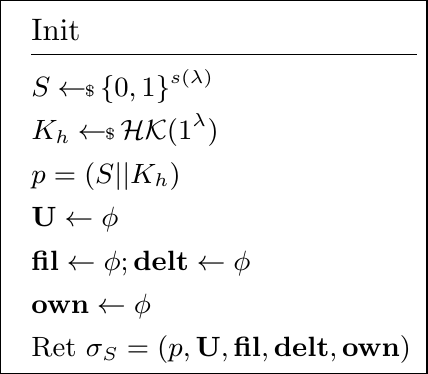
\includegraphics[scale=0.5]{init}    
	\caption{The $\mathsf{Init}$ procedure. This will set up the server, create empty databases $\mathsf{fil}$ and $\mathsf{own}$ and runs $\mathcal{P}(1^{\lambda})$. $\mathsf{fil}$ stores the encrypted files uploaded by the client and is indexed by the tag. $\mathsf{own}$ stores the ownership information and associates with each client, the tag of the files uploaded by the client.}
\end{figure}

\noindent
The $\mathsf{Reg}$ protocol registers a new client with the server. The server picks a unique client identifier and returns it to the client.

\begin{figure}[H]
	\centering
	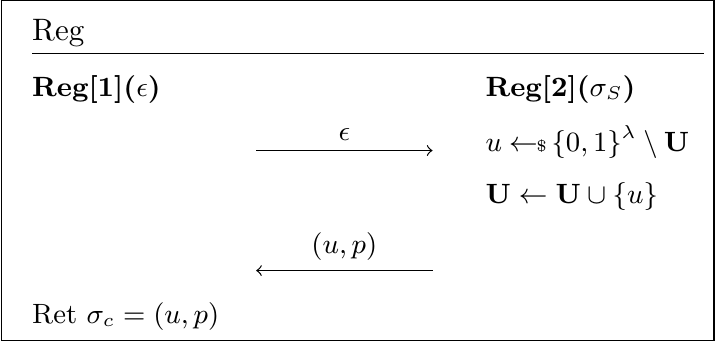
\includegraphics[scale=0.5]{reg}
	\caption{The $\mathsf{Reg}$ protocol. This returns the client parameters $\sigma_c$ which includes the client credentials and the keys generated in \textsc{Init}}	
\end{figure}

\begin{figure}[H]
	\centering
	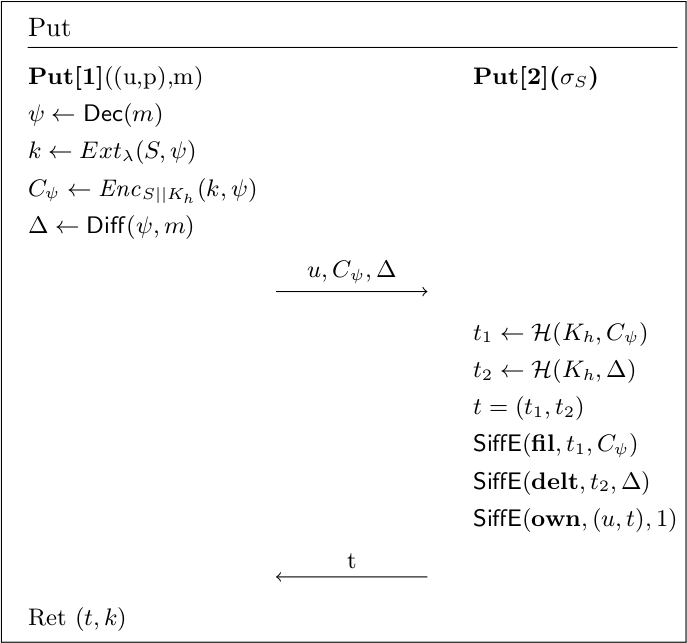
\includegraphics[scale=0.5]{put}
	\caption{The $\mathsf{Put}$ protocol. \textbf{fil}, \textbf{delt} and \textbf{own} tables are immutable. Here the $\Delta$ is stored in $\textbf{delt}$ table and $\textbf{own}$ table stores a $1$ to show that the client with credentials $u$ owns the file with tag $t$}
	\label{fig:put}
\end{figure}

\noindent
In the $\mathsf{Put}$ protocol, the message $m$ is first mapped to its codeword $\psi$. $\Delta = \mathsf{Diff}(\psi, m)$ is computed. The client then sends $(\mathsf{E}(k,\psi), \Delta)$ to the server. The server hashes $\psi$ and $\Delta$ to get the tag $t = (t_1 = \mathcal{H}(K_h, \psi), t_2 = \mathcal{H}(K_h, \Delta))$. The message is finally stored in the $\textbf{fil}$ and $\textbf{delt}$ tables. $\textbf{fil}[t_1] = C_\psi$ and $\textbf{delt}[t_2] = \Delta$. The ownership table is also updated to reflect this. $\textbf{own}[u,t]=1$. If another client (with credentials $u'$) tries to upload the same file $m$, then the server only needs to update it on the ownership table. $\textbf{own}[u',t]=1$.

\begin{figure}[H]
	\centering
	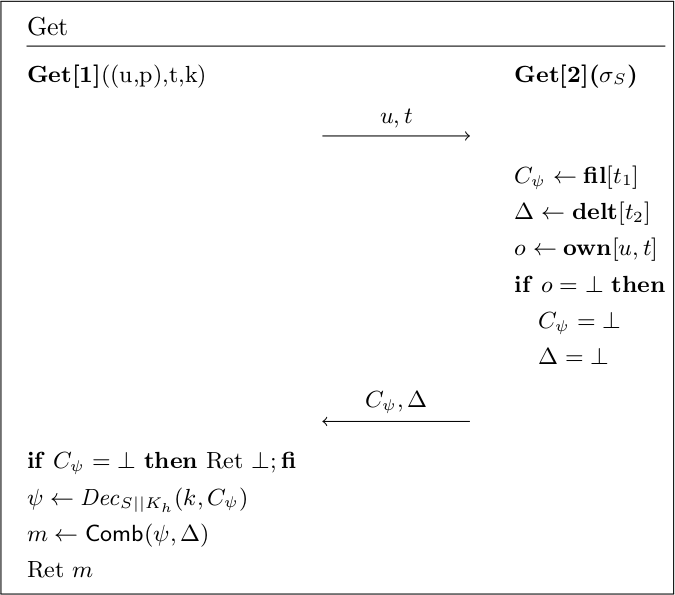
\includegraphics[scale=0.5]{get}
	\caption{The $\mathsf{Get}$ protocol.}
	\label{fig:get}
\end{figure}

\noindent
In the $\mathsf{Get}$ protocol, client sends the tag $t$ and credentials to the server. The server verifies if the client owns the file  by checking the ownership table and if it does, returns $C_\psi$ and $\Delta$. The client decrypts $C_psi$ to get $\psi$ and applies $\mathsf{Comb}(\psi, \Delta)$ to get back $m$.
